\chapter{\leavevmode\newline TTWR state space analysis}
\chaptermark{TTWR state space analysis}
\label{chap:TTWR state space analysis}

This chapter outlines the main focus of the research, detailing the definition of the TTWR state space and its controllability analysis. The study employs a kinematic truck-trailer vehicle model to represent a simulation vehicle operating at low speeds without tire slip. While a comprehensive model might encompass vehicle dynamics, such as load transfer and tire slip, this research primarily centers on the kinematic aspects for low speed parking scenarios. The chapter concludes by addressing the limitations of the TTWR model and the common methods to avoid such issue.

\section{TTWR kinematics state space}

Previous research \parencite{sorge2019motion}\parencite{liu2019minimum} has provided various physical models for vehicle state analysis, including both kinematic and dynamic state models. The choice of model depends on the desired level of accuracy and the specific operating conditions. For high-speed driving tasks, the dynamic factors play a significant role in motion planning and vehicle control; however, in low-speed driving scenarios, the kinematic constraints have a greater influence on the motion behavior of the TTWR system. Since the TTWR reverse parking task is operated in low-speed driving conditions, the system model is established based on the kinematic relations. In this paper, we utilized the Ackermann chassis vehicle as the host vehicle, and the trailer employed a single-axle chassis for the TTWR system. The two vehicles in the system are linked by the hitch ball, which is a unique pivoting point. The pivot point enables the interconnected vehicles to execute relative rotational motion between each other. From a mechanical structure perspective, the tractor and the trailer can be regarded as two separate rigid bodies. The vehicle body structure exhibits symmetry with respect to the axis, with the left and right sides being symmetrical. On flat non-slippery ground and under low-speed driving, the side-slip caused by tires and control effect delay caused by mechanical or electrical units can be neglected\parencite{lei2021research}. In Table \ref{table: ttwr system states}, the major parameters of the TTWR system are listed.

\begin{table}
\centering
\caption{The TTWR system states}
\setlength{\tabcolsep}{12pt}
\begin{tabular}{|p{3cm}|p{9cm}|}
\hline
Parameters& 
Descriptions  \\
\hline
$x_1 $& 
The lateral position of the host vehicle \\
$y_1$& 
The longitudinal position of the host vehicle \\
$\theta_1$& 
The yaw angle of the trailer \\
$x_2 $& 
The lateral position of the trailer \\
$y_2$& 
The longitudinal position of the trailer \\
$\theta_2$& 
The yaw angle of the host vehicle \\
$\phi $& 
The host-trailer angle \\
$v$& 
The longitudinal velocity of host vehicle \\
$\delta $& 
The steering angle of host vehicle \\
$L_1$& 
The host vehicle wheelbase length \\
$L_2$& 
The rear overhang of the host vehicle from the rear axle to the hitch point \\
$L_3$& 
The overhang of the trailer from the the hitch to trailer axle \\
\hline
\end{tabular}
\label{table: ttwr system states}
\end{table}

\begin{figure}[h]
\centering
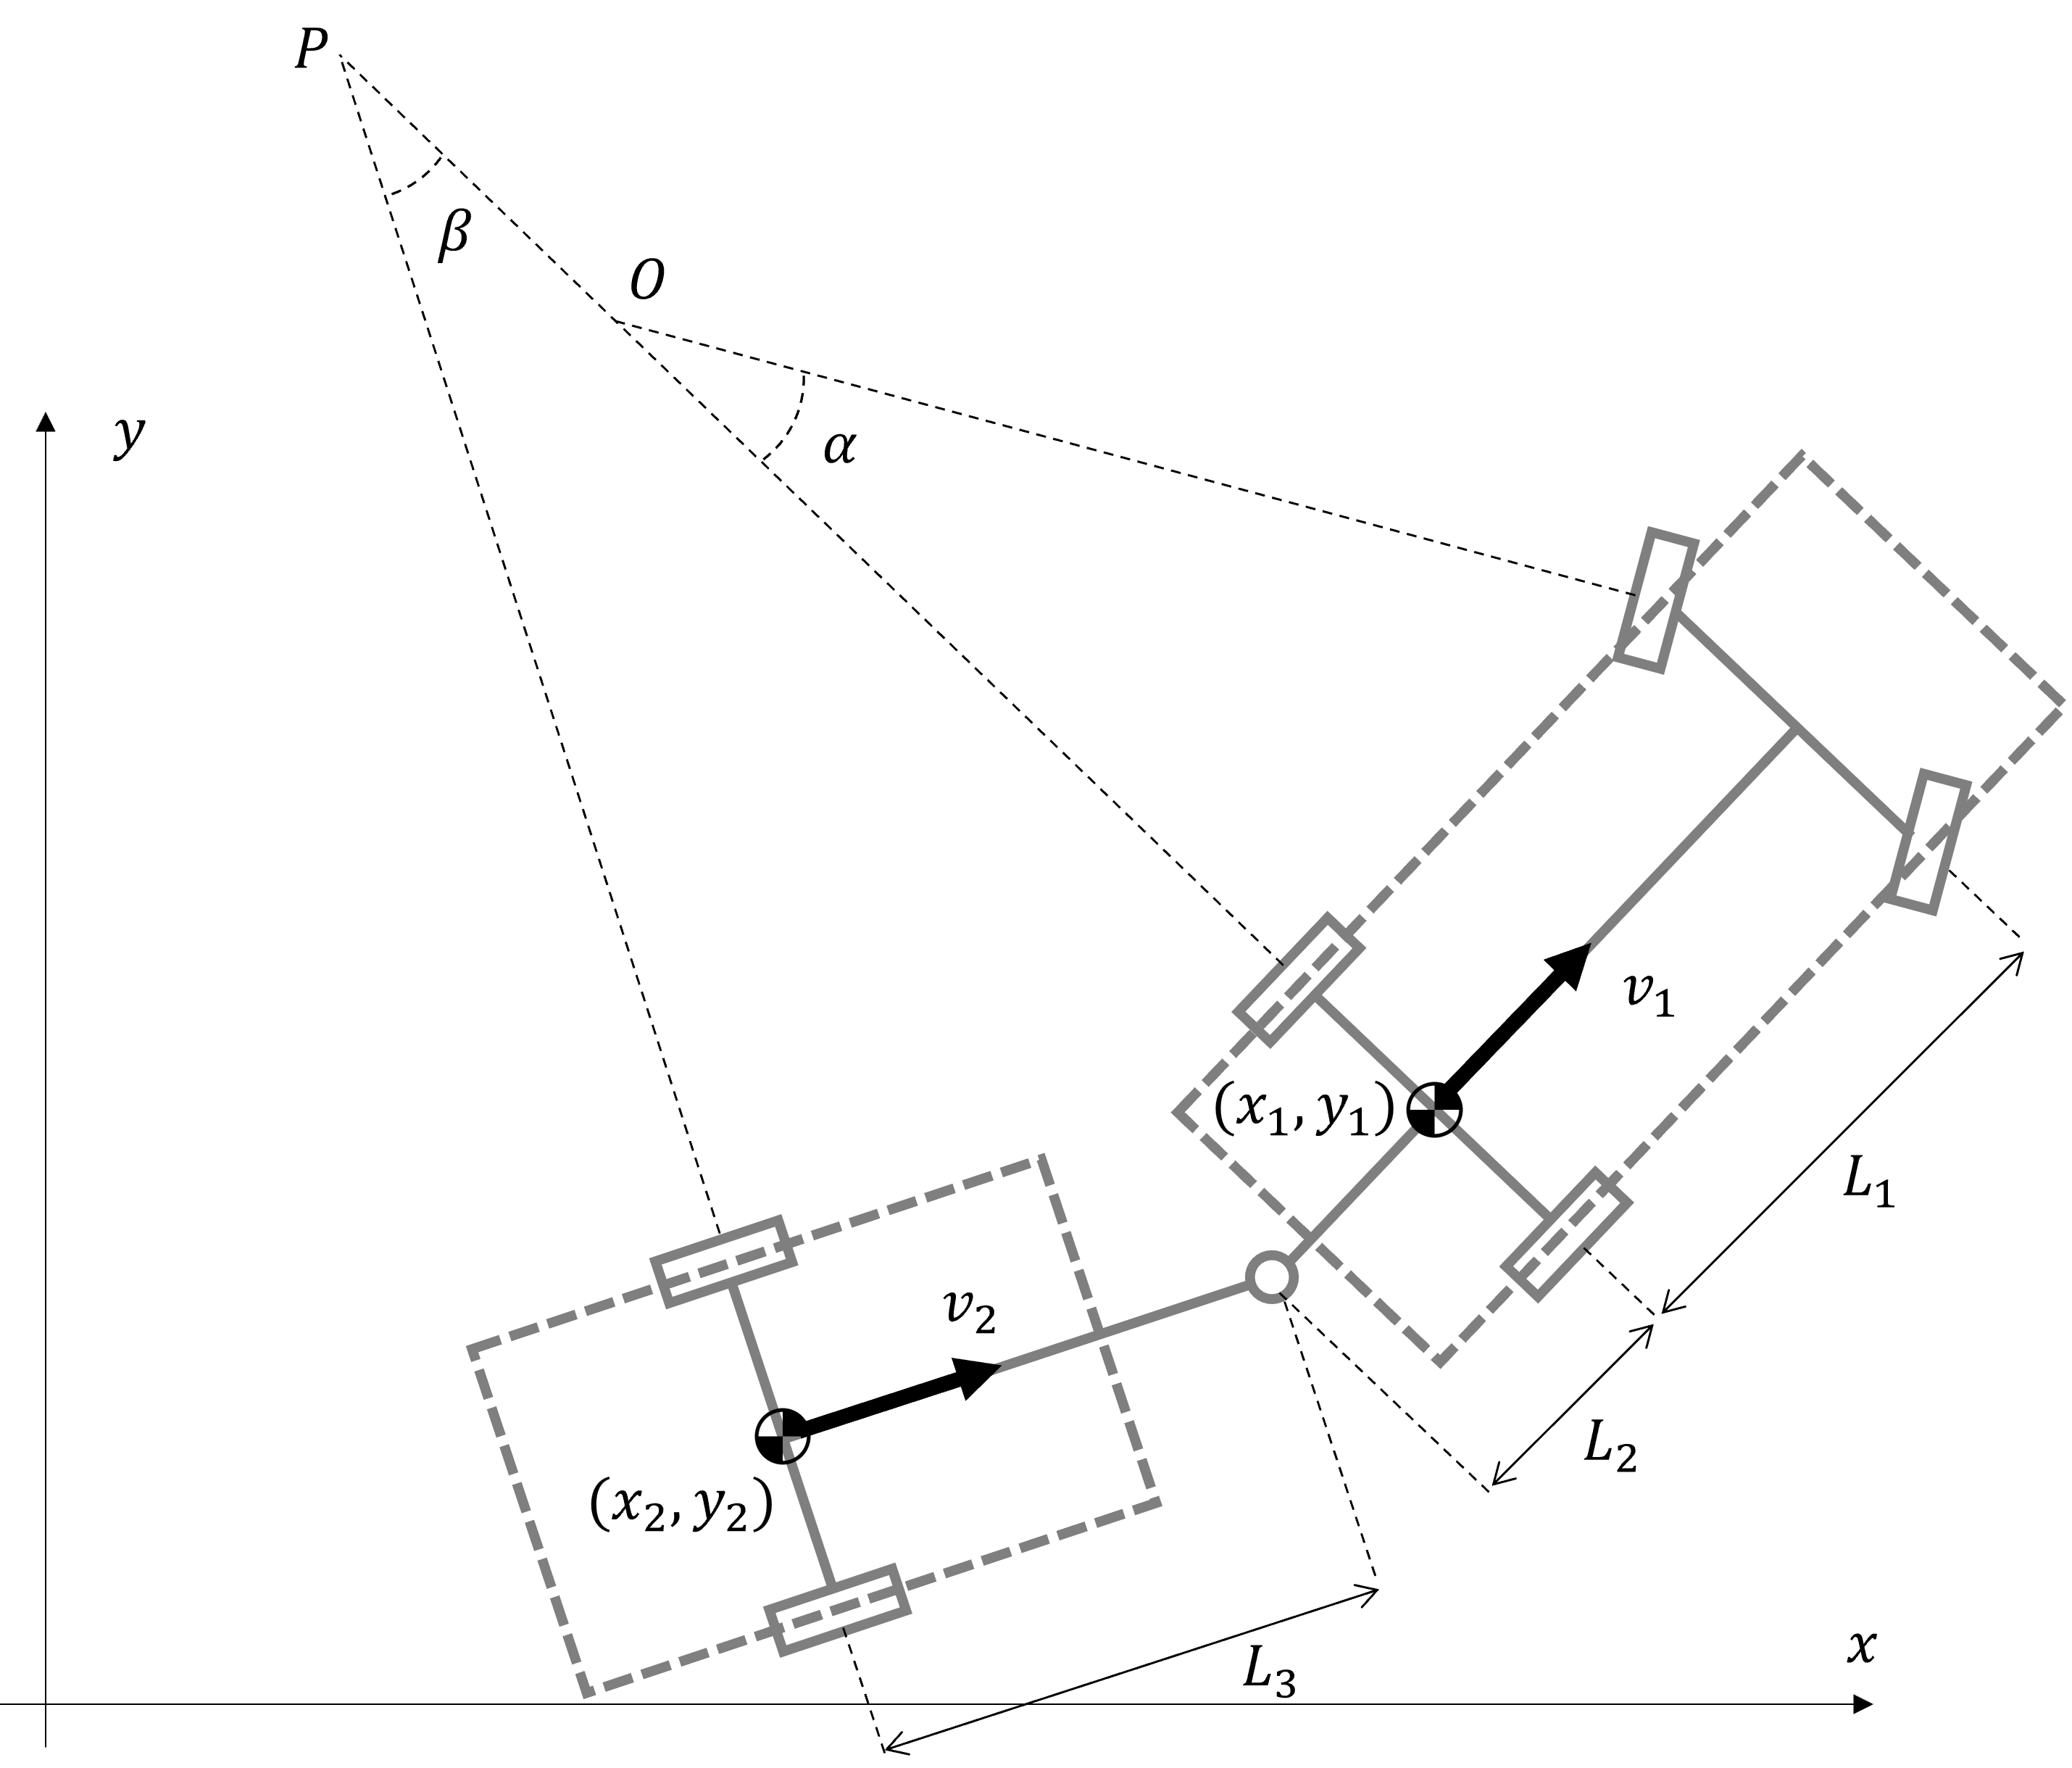
\includegraphics[scale=0.35]{fig/full_track_vehicle_model.png}
\caption{Kinematic full-track model of TTWR}
\label{fig:full track kinematics mdoel}
\end{figure}

This state-space model of TTWR in this paper is illustrated in Figure \ref{fig:full track kinematics mdoel}, where the trailer has a single axle and a conventional overrun braking system. The assumptions for the TTWR system are as summarized as follows: 

\begin{itemize}
  \item The system has a unique pivoting point, known as the hitch, which is essential in yielding the unstable equilibrium point during reverse driving.
  \item The system is defined on a flat surface and without slide slip in the kinematics model and simulation environment.
  \item The trailer has a uniformly distributed mass.
\end{itemize}

Because all the perception values are received in the vehicle coordinate, it is essential to build the reference point coordinate transformation between the vehicle coordinate and the world coordinate. In this paper, only the translation from trailer coordinate to world coordinate is explained, because host coordinate transformation also follows a similar computation.

Under the trailer coordinate, the reference points coordinates can be expressed as:
\begin{equation}
P_2=\left[\begin{array}{cccc}
x_{21} & x_{22} & \cdots & x_{2n} \\
y_{21} & y_{22} & \cdots & y_{2n}
\end{array}\right]
\label{eq: reference point matrix}
\end{equation}
where $P_2$ is the coordinate vector matrix, each column vector of the matrix represents a reference point (e.g. surrounding obstacle detections, trailer corner coordinate and et al.) under the trailer coordinate system. $\left(x_{21}, x_{22}, \ldots, x_{2n}\right)$ and $\left(y_{21}, y_{22}, \ldots, y_{2n}\right)$ are X-coordinate and the Y-coordinate values respectively.

In linear algebra, the rotation matrix $R_\text{world}$ and the translation matrix $T_\text{world}$ can be known as:
\begin{equation}
\operatorname{R}_\text{world} = \left[\begin{array}{ccc}
\cos \theta_2 & -\sin \theta_2 \\
\sin \theta_2 & \cos \theta_2
\end{array}\right]
\label{eq: rotation matrix}
\end{equation}

\begin{equation}
\operatorname{T}_\text{world} =\left[\begin{array}{ccc}
t_{x2} & t_{y2}
\end{array}\right]^T
\label{eq: translation matrix}
\end{equation}
where the $(x_2, y_2)$ are the origin point of the trailer coordinate on the trailer rear axle center, and then the coordinate vector translation from trailer coordinate to world coordinate can be expressed as:
\begin{equation}
P_\text{world}=\operatorname{R}_\text{world} * P_2 + \operatorname{T}_\text{world}
\label{eq: transform coordinate 2 to coordinate world}
\end{equation}

\begin{figure}[h]
\centering
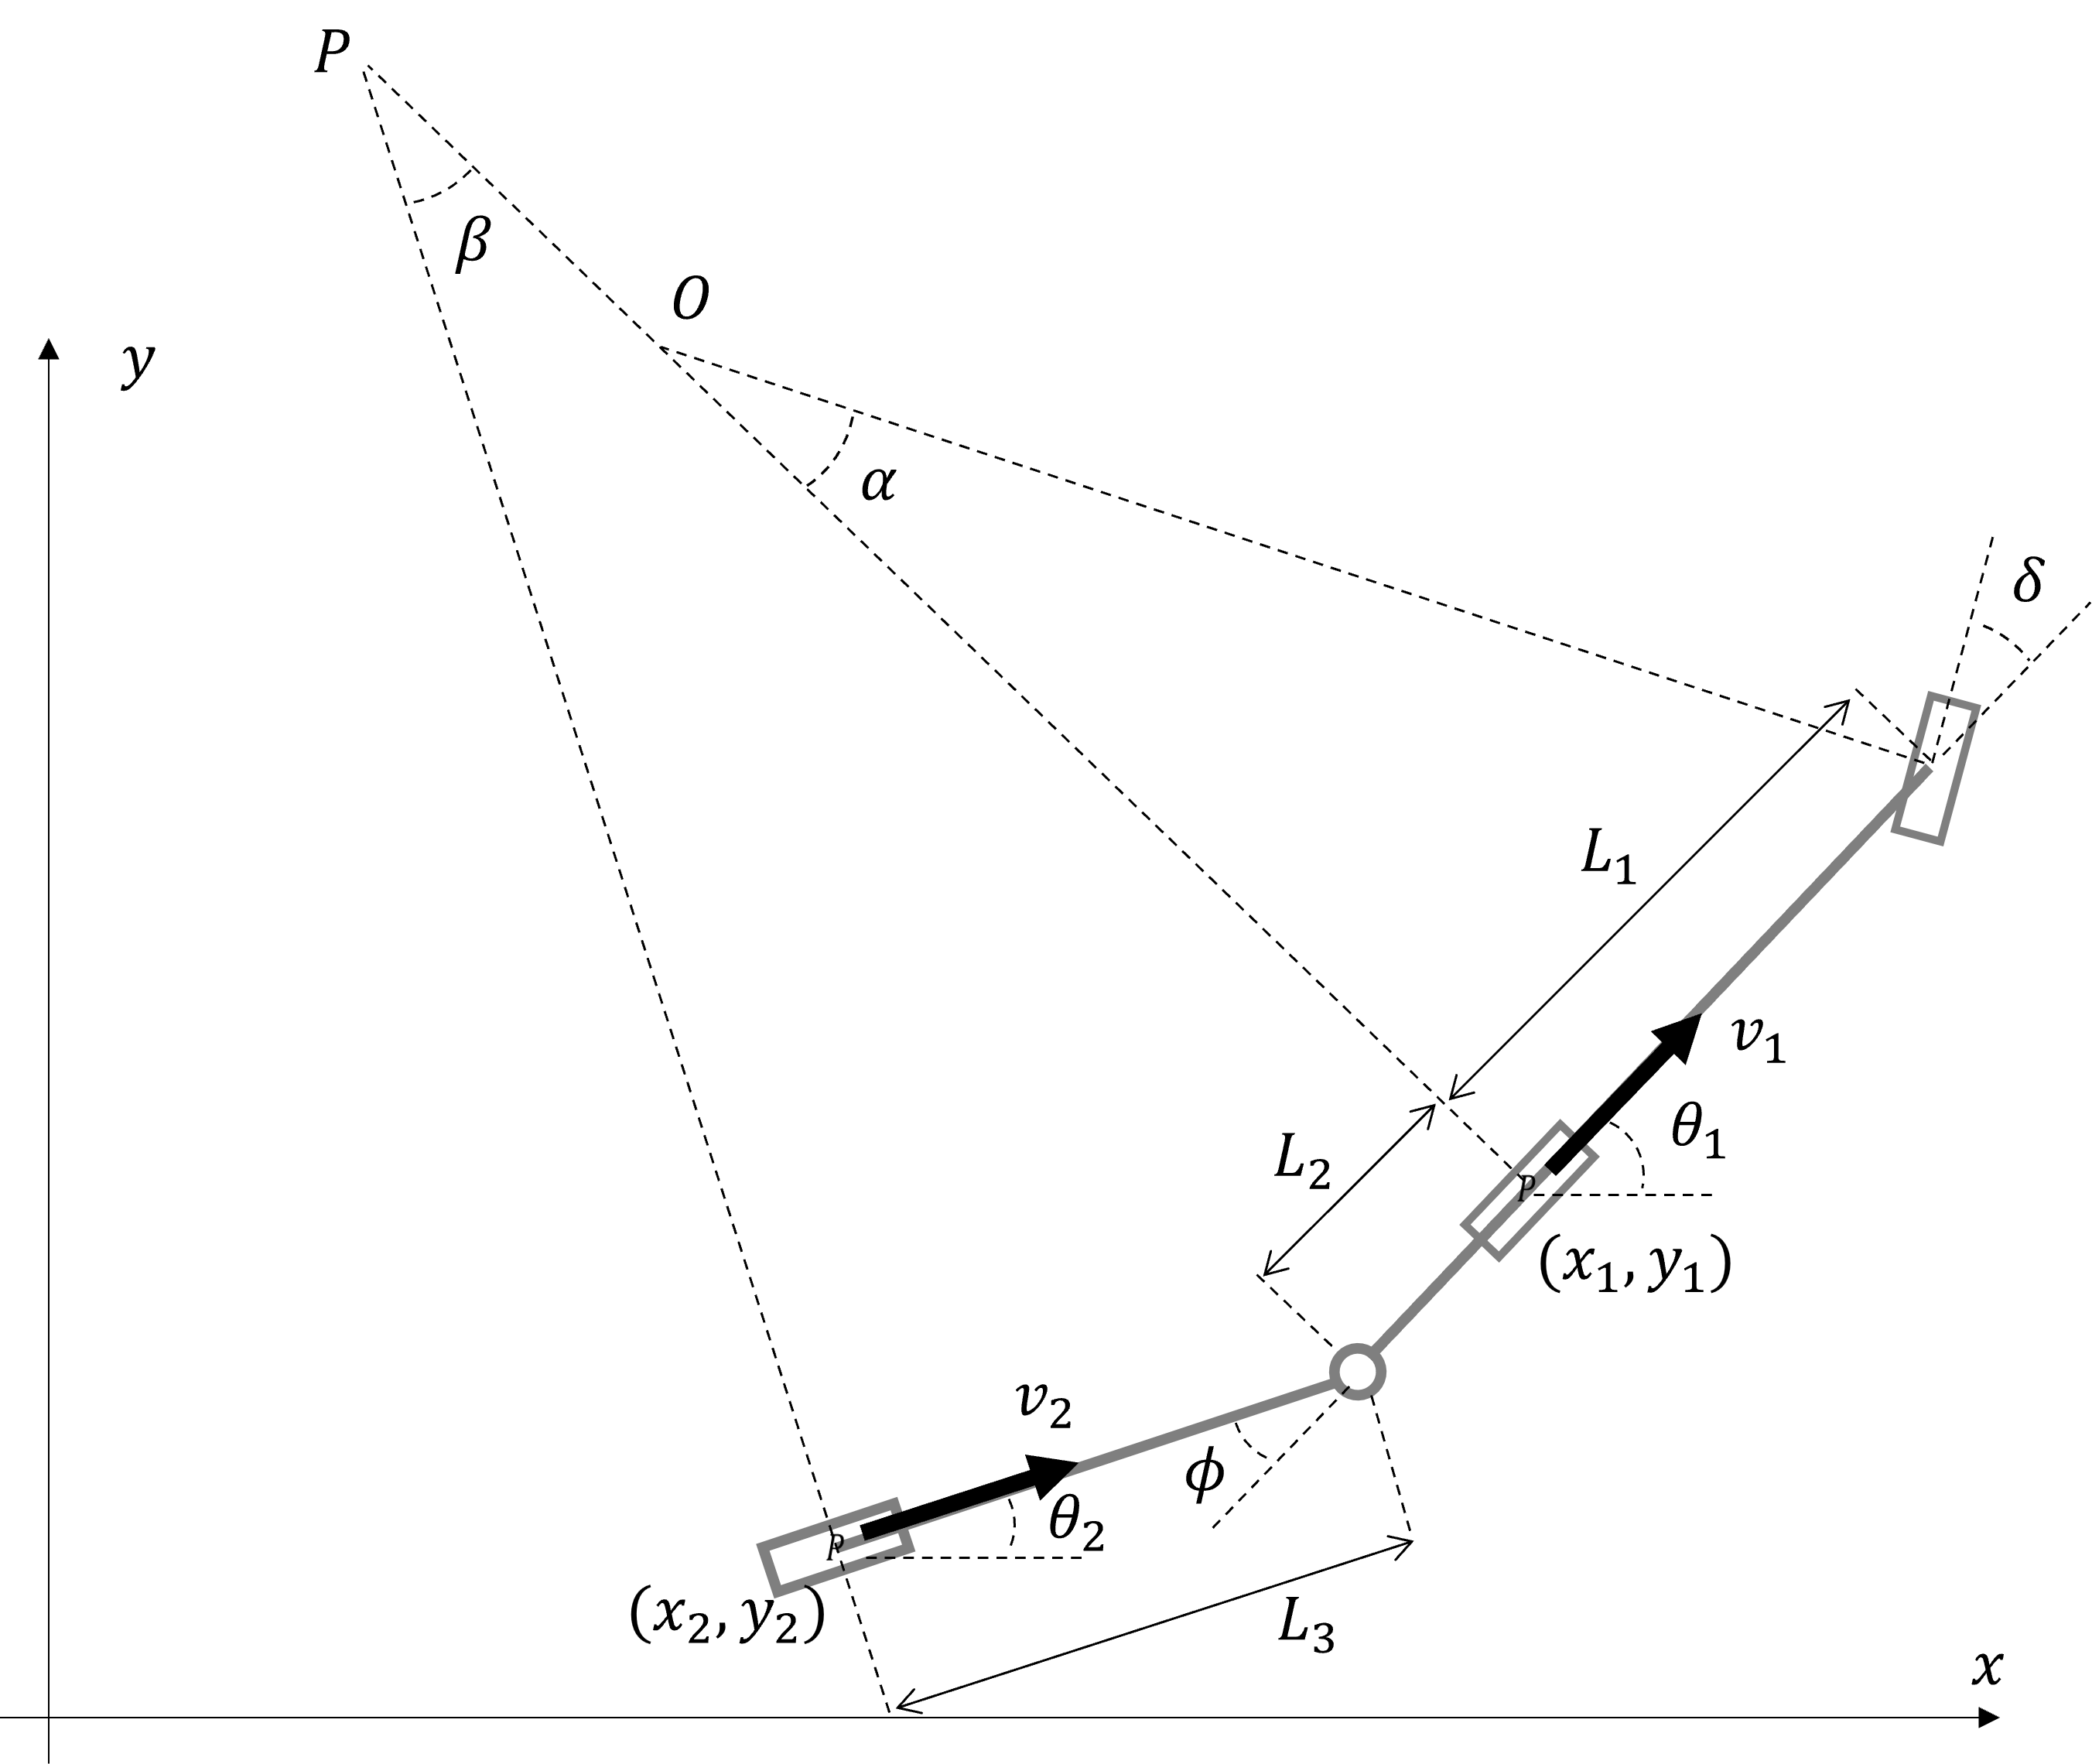
\includegraphics[scale=0.35]{fig/bicycle_vehicle_model.png}
\caption{Simplified bicycle kinematic model of TTWR}
\label{fig:Simplified bicycle kinematic model of TTWR}
\end{figure}

In the world coordinate, the host vehicle state model is referred to as the front wheel Ackerman steering model, which allows control of the front wheel orientation relative to the heading of the vehicle. Due to limitations on the available computational power, vehicle dynamics are often highly simplified at the simulation phase \parencite{polack2017kinematic}. Because the state model in this paper is carried out at low speed and with the assumption of an ideally flat environment, the full track model represented in Figure \ref{fig:full track kinematics mdoel} can be further simplified as the kinematic bicycle model in Figure \ref{fig:Simplified bicycle kinematic model of TTWR}, and the host vehicle kinematic equation can be expressed as:
\begin{equation} \dot{x}_1=v \cos{\theta_1} \label{eq: x1}\end{equation}
\begin{equation} \dot{y}_1=v \sin{\theta_1} \label{eq: y1}\end{equation}
\begin{equation} \dot{\theta}_1 = \frac{v}{L_1}\tan{\delta} \label{eq: theta1}\end{equation}

The kinematic model of the trailer can be derived by propagating the state space of the host vehicle, as the trailer's kinematics are influenced by the maneuver of the host vehicle. The longitudinal speed of the trailer can be estimated by projecting the normal and longitudinal speed of the host vehicle onto the longitudinal axis of the trailer at the hitch point. Following the bicycle kinematic model, the states $[x_2, y_2, \theta_2]^T$ of the trailer can be expressed as:
\begin{equation} \dot{x}_2 = v \cos{\phi} (1 - \frac{L_2}{L_1}\tan{\phi}\tan{\delta})\cos{\theta_2} \label{eq: x2}\end{equation}
\begin{equation} \dot{y}_2 = v \cos{\phi} (1 - \frac{L_2}{L_1}\tan{\phi}\tan{\delta})\sin{\theta_2} \label{eq: y2}\end{equation}
\begin{equation} \dot{\theta}_2 = -v (\frac{\sin{\phi}}{L_3} + \frac{L_2}{L_1 L_3}\cos{\phi}\tan{\delta} ) \label{eq: theta2}\end{equation}

To evaluate the threat of jack-knifing, the host-trailer angle is also required for trailer state prediction, which is defined by the difference between Eqn.\ref{eq: theta2} and Eqn.\ref{eq: theta1}:
\begin{equation} 
\dot{\phi} = -\frac{v}{L_3}\sin{\phi} - \frac{v}{L_1} ( 1 + \frac{L_2 \cos{\phi}}{L_3}) \tan{\delta} 
\label{eq: phi}
\end{equation}

During reverse driving, the host-trailer system is limited to one degree of freedom in control, which is the host vehicle steering input, the system control is designed to minimize mainly the trailer's tracking error. So, the control reference variables are defined by the trailer’s rear axle center position $(x_2, y_2)$, and heading ${\theta}_2$ compared with the parking slot's reference position  $(x_{goal}, y_{goal})$, and heading angle ${\theta}_{goal}$.

\section{TTWR system physical constrains}

Jack-knifing is a significant constrain in the dynamics of truck trailer wheeled robot systems. It occurs when the angle between the truck and trailer reaches a point where control over the trailer's direction is lost during reverse motion. Rather than aligning with the desired trajectory, the angle continues to grow, culminating in the trailer contacting the tractor. At this stage, the system enters an uncontrollable state, representing a critical failure mode in the control of tractor-trailer systems. Abraham \parencite{abraham2013trailer} provides an explanation for the phenomenon of jack-knifing, identifying it as a situation where the trailer's angular velocity surpasses that of the towing vehicle, even when maximum steering input is applied. Geometrically, this is interpreted as the trailer's center of rotation moving beyond the corresponding point of the towing vehicle. The critical threshold for jack-knifing is reached when these two centers of rotation coincide, leading to a loss of control over the trailer's direction.

\section{Controllability}

Controllability is an important characteristic for the control system, which significantly impacts various control challenges, including stabilizing unstable systems through feedback and optimizing control. Complete state controllability refers to the capacity of an external input (consisting of control variables) to move the system's internal states from any starting states to any final states within a finite time frame. In simpler terms, a system is considered controllable if there exists a control input that enables the transition from any initial state to any desired final state within a specified time interval.

Consider the continuous linear system
\begin{equation}
\label{eqn: lti system states}
\begin{aligned}
& \dot{{x}}(t)=A(t) {x}(t)+B(t) {u}(t) \\
& {y}(t)=C(t) {x}(t)+D(t) {u}(t) .
\end{aligned}
\end{equation}
where ${x}(t_0)=x^0$ is the initial states when the system starts.

The state pair sets $(x, u)$ which solve Equation \ref{eqn: lti system states} for by setting the initial states $\left(t_0, x^0\right)$ is called the behaviour $\mathcal{B}_{(A, B)}$ of Equation \ref{eqn: lti system states}:
\begin{equation}
\mathcal{B}_{(A, B)}:=\left\{(x, u) \in X \times U \mid \exists\left(t_0, x^0\right) \in \mathbb{R} \times \mathbb{R}^n, \quad x(\cdot)=x\left(\cdot ; t_0, x^0, u\right)\right\}
\end{equation}

Here, $X$ is a suitable space of functions such that
\begin{equation}
\left\{x\left(\cdot ; t_0, x^0, u\right) \mid\left(t_0, x^0\right) \in \mathbb{R} \times \mathbb{R}^n, \quad u \in U\right\} \subseteq X .
\end{equation}

Regarding the concept of controllability, the system $(A, B)$ is called 
\begin{itemize}
    \item Reachable at time $T>0$ if for all $x^1 \in \mathbb{R}^n$ there exists $(x, u) \in \mathcal{B}_{(A, B)}$ such that $x(0)=0$ and $x(T)=x^1$,
    \item Controllable at time $T$ if for all $x^0, x^1 \in \mathbb{R}^n$ there exists $(x, u) \in \mathcal{B}_{(A, B)}$ such that $x(0)=x^0$ and $x(T)=x^1$,
    \item Null-controllable at time $T$ if for all $x^0 \in \mathbb{R}^n$ there exists $(x, u) \in \mathcal{B}_{(A, B)}$ such that $x(0)=x^0$ and $x(T)=0$.
\end{itemize}

To determine which states can be more or less easily controlled, it is required to examine the eigen decomposition of the Controllability Gramian. This process reveals insights into the relationships between the system states and how they respond to the control inputs. The Controllability Gramian $W\left(t_0, t_1\right)$ is defined as:
\begin{equation}
\label{eqn_controllability_gramian}
W\left(t_0, t_1\right)=\int_{t_0}^{t_1} \phi\left(t_0, t\right) B(t) B(t)^T \phi\left(t_0, t\right)^T d t
\end{equation}
where $\phi$ is the state-transition matrix. 

The Equation \ref{eqn_controllability_gramian} means if there exists a control $u$ from state $x_0$ at time $t_0$ to state $x_1$ at time $t_1>t_0$ if and only if $x_1-\phi\left(t_0, t_1\right) x_0$ is in the column space of the Controllability Gramian.

In fact, if $\eta_0$ is a solution to $W\left(t_0, t_1\right) \eta=x_1-\phi\left(t_0, t_1\right) x_0$ then a control given by $u(t)=-B(t)^T \phi\left(t_0, t\right)^T \eta_0$ would make the desired transfer.

Note that the matrix $W$ defined as above has the following properties:
\begin{itemize}
\item  $W\left(t_0, t_1\right)$ is symmetric
\item $W\left(t_0, t_1\right)$ is positive semidefinite for $t_1 \geq t_0$
\item $W\left(t_0, t_1\right)$ satisfies the linear matrix differential equation
\begin{equation}
\frac{d}{d t} W\left(t, t_1\right)=A(t) W\left(t, t_1\right)+W\left(t, t_1\right) A(t)^T-B(t) B(t)^T, W\left(t_1, t_1\right)=0
\end{equation}
\item $W\left(t_0, t_1\right)$ satisfies the equation \parencite{brockett2015finite}
\begin{equation}
W\left(t_0, t_1\right)=W\left(t_0, t\right)+\phi\left(t_0, t\right) W\left(t, t_1\right) \phi\left(t_0, t\right)^{T}
\end{equation}
\end{itemize}

Gramians are also useful to determine the minimum-energy control ${u}(t)$ required to navigate the system to ${x}\left(t_f\right)$ at time $t_f$ from ${x}(0)=0$ \parencite{brunton2022data}:
\begin{equation}
{u}(t)={B}^*\left(e^{{A}\left(t_f-t\right)}\right)^* {W}_c\left(t_f\right)^{-1} {x}\left(t_f\right) .
\end{equation}

The total energy expended by this control law is given by
\begin{equation}
\int_0^{t_f}\|{u}(\tau)\|^2 d \tau={x}^* {W}_c\left(t_f\right)^{-1} {x} .
\end{equation}

If the controllability matrix is close to singular, more actuation enger will be required to drive the states to certian direction. On the other hand, if the eigenvalues of ${W}_c$ are all large, then the system is easily controlled.

It is generally impractical to compute the Gramians directly using Equation \ref{eqn_controllability_gramian}. Instead, the Controllablity Gramian is the solution to the following Lyapunov equation:
\begin{equation}
{A W}_c+{W}_c {A}^*+{B B}^*={0},
\end{equation}
while the observability Gramian is the solution to
\begin{equation}
{A}^* {W}_o+{W}_o {A}+{C}^* {C}={0} .
\end{equation}

Obtaining Gramians by solving a Lyapunov equation is typically quite expensive for high-dimensional systems. Instead of this computationally demanding approach, Gramians are frequently approximated empirically. This approximation is achieved using snapshot data gathered from both the direct system and the adjoint system, providing a more efficient means to estimate these important mathematical constructs.

In practice, the Controllability Gramian requires the integration of a system's state-transition matrix. For a simpler assessment of system controllability, a rank condition can be used that is similar to the Kalman rank condition found in time-invariant systems, which shows that the Controllability of a LTI system is determined entirely by the column space of the controllability matrix $\mathcal{C}$ :
\begin{equation}
\mathcal{C}=\left[\begin{array}{lllll}
{B} & {AB} & {A}^2 {~B} & \cdots & {A}^{n-1} {~B}
\end{array}\right] .
\end{equation}

If the matrix $\mathcal{C}$ has $n$ linearly independent columns, meaning that it spans all of $\mathbb{R}^n$, then the system is considered controllable. The span of the columns of the controllability matrix$\mathcal{C}$ forms a Krylov subspace, which identifies the directions in $\mathbb{R}^n$ that can be manipulated with control. Consequently, controllability not only implies the possibility of arbitrary eigenvalue placement but also ensures that any state $\xi \in \mathbb{R}^n$  can be reached within a finite time using a specific actuation signal ${u}(t)$ \parencite{brunton2022data}.

In general, for a system $(A, B)$ the following statements are equivalent:
\begin{itemize}
    \item There exists $T>0$ such that $(A, B)$ is controllable at time $T$.
    \item $\operatorname{im}(K(A, B))=\mathbb{R}^n$
    \item $\operatorname{rank}(K(A, B))=n$
    \item For all $T>0$ the system $(A, B)$ is controllable at time $T$. We say that $(A, B)$ is controllable.
\end{itemize}

\section{TTWR system analysis}
\label{section: ttwr system analysis}

To identify the properties and conditions of the truck trailer system, its equilibrium, observability, and controllability are analyzed. Let $ x = [y_2, \theta_2, \phi]^\intercal$ be the trailer states obtained from Equation \ref{eq: x2} - \ref{eq: theta2} by neglecting the longitudinal component $x_3$, the state space model can be written as \parencite{altafini2001feedback}:

\begin{equation} \dot{x} = v ( \mathcal{A} ( x ) + \mathcal{B} (x;\delta)) \label{eq: state space model}\end{equation}

The equilibrium state of $x$ is the origin $x_e = 0$, and we can derive the trailer equilibrium state from Equation \ref{eq: phi}: 

\begin{equation} x_e = \{(y_2, \theta_2, \phi) \mid \delta = 0, y_2 \in \mathbb{R}, \theta_2 \in [-\pi, \pi), \phi = 0\} \label{eq: equilibrium states}\end{equation}

The equilibrium set indicates during reverse driving, the trailer system is in an equilibrium state when the host vehicle and trailer are aligned in either direction, and there should be no steering angle input given by the host vehicle.

To examine the internal asymptotic stability, we substitute $\delta = 0$ into Equation 8, resulting in the following equation:
\begin{equation} 
\dot{x} = v ( \mathcal{A} x + \mathcal{B} \delta)
\label{eq: state space when delta is 0}
\end{equation}
where
\begin{equation} 
\mathcal{A} = \begin{bmatrix}
0 & 1 & 0 \\
0 & 0 & -\frac{1}{L_3} \\
0 & 0 & -\frac{1}{L_3}
\end{bmatrix} 
\mathcal{B}= \begin{bmatrix}
0 \\
\frac{L_2}{L_1L_3} \\
-\frac{L_3+L_2}{L_1L_3}
\end{bmatrix} \label{eq: state transfer matrix linearization}\end{equation}

By using the Cayley-Hamilton theorem, the controllability matrix $\mathcal{C} = [B, AB, AAB]$ is row full rank for state space in Equation \ref{eq: state space when delta is 0}, which shows the host-trailer system to be controllable out of the singular locus \parencite{altafini1999controllability}, and the origin of the nonlinear system can be made an asymptotically stable equilibrium by state feedback.


\begin{figure}
     \centering
     \begin{subfigure}[b]{0.8\textwidth}
         \centering
         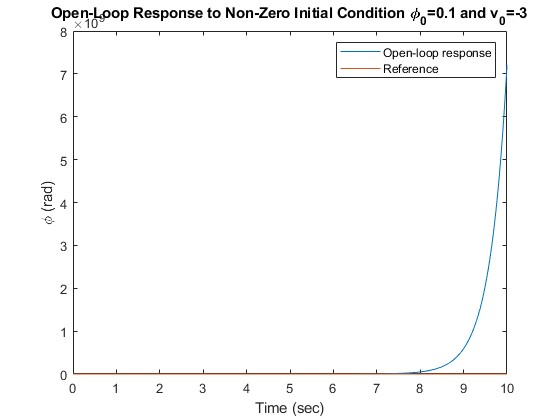
\includegraphics[width=0.7\linewidth]{fig/openloop_respond/negative velo openloop response - Copy.jpg}
         \caption{The positive velocity indicates stable system behaviour when teh TTWR can correct its $\Phi$ value}
     \end{subfigure}
     \vfill 
     \begin{subfigure}[b]{0.8\textwidth}
         \centering
         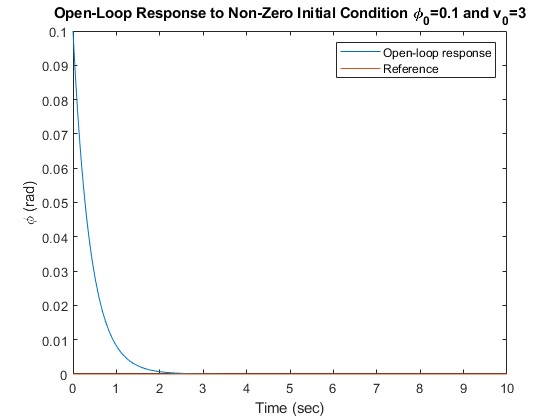
\includegraphics[width=0.7\linewidth]{fig/openloop_respond/positive velo openloop response - Copy.jpg}
         \caption{The negative velocity will cause unstable system performance, the $\Phi$ angle keeps increasing until reach jacknifing}
     \end{subfigure}
    \caption{Open loop respond comparison between the positive and negative truck velocity}
\end{figure}